\documentclass[twocolumn,10pt]{article}

\usepackage[french]{babel}
\usepackage[utf8]{inputenc}
\usepackage[T1]{fontenc}
\usepackage{amsmath}
\usepackage{graphicx}
\usepackage{booktabs}
\usepackage{float}
\usepackage{geometry}
\usepackage{caption}
\usepackage{hyperref}

\geometry{margin=1.75cm,top=19mm,bottom=18mm,columnsep=15pt}
\captionsetup{font=small,labelfont=bf}
\setlength{\parindent}{0pt}
\setlength{\parskip}{2pt}
\setlength{\textfloatsep}{5pt}
\setlength{\floatsep}{5pt}
\setlength{\intextsep}{5pt}

\title{Dans quelle mesure les variables de contexte permettent-elles d'expliquer les différences de réussite scolaire et de prédire les résultats des élèves ?}
\author{Groupe D1\_B}
\date{}

\begin{document}

\maketitle
\vspace{-0.4em}

\begin{abstract}
Nous étudions le jeu de données \emph{Student Performance} afin de déterminer si les variables de contexte permettent d'expliquer ou de prédire le niveau scolaire. Les notes intermédiaires \texttt{G1} et \texttt{G2} sont volontairement retirées pour éviter une prédiction triviale de \texttt{G3}. La démarche combine ACP, arbres de décision, régression logistique et analyse discriminante. Les résultats montrent un signal réel mais limité: les variables de contexte aident à repérer des facteurs associés à la réussite, mais ne suffisent pas à prédire précisément la note finale ni à séparer nettement réussite et échec.
\end{abstract}

\section{Objectif de l'étude}

Le jeu de données contient des informations scolaires, familiales et comportementales sur des élèves suivis en mathématiques et en portugais. L'objectif n'est pas seulement de décrire les notes, mais de tester si des variables comme \texttt{age}, \texttt{Medu}, \texttt{Fedu}, \texttt{studytime}, \texttt{failures}, \texttt{goout}, \texttt{Dalc}, \texttt{Walc}, \texttt{absences} ou \texttt{higher} permettent d'expliquer les différences de niveau.

Pour éviter un modèle artificiellement performant, les notes intermédiaires \texttt{G1} et \texttt{G2} ne sont pas utilisées dans les modèles prédictifs. On distingue deux questions: peut-on prédire précisément la note finale \texttt{G3} ? Peut-on au moins classer les élèves en réussite ou en échec, avec la règle \texttt{G3 >= 10} ?

\section{Données et préparation}

Les deux tables contiennent 395 élèves en mathématiques et 649 élèves en portugais. Elles sont fusionnées sur des variables communes d'identification et de contexte; la fusion conserve 382 élèves communs aux deux matières.

Dans les données fusionnées, le suffixe \texttt{.x} correspond aux mathématiques et le suffixe \texttt{.y} au portugais. Ainsi, \texttt{G3.x} désigne la note finale en mathématiques et \texttt{G3.y} celle en portugais.

Pour les modèles prédictifs, les notes intermédiaires sont retirées. On conserve donc les variables de contexte: âge, sexe, absences, temps d'étude, éducation des parents, soutien scolaire, sorties, consommation d'alcool, souhait de poursuivre des études supérieures, etc.
Cependant pour les différents modèles nous nous sommes concentrés sur les notes des élèves de maths
\section{Profils de niveau et ACP descriptive}

Une première analyse construit trois profils d'élèves à partir des notes finales en mathématiques et en portugais. La figure~\ref{fig:kmeans} montre des groupes interprétables: élèves en difficulté, élèves moyens et élèves avec de bons résultats. Les moyennes des groupes sont environ $(2{,}81;9{,}68)$, $(10{,}56;11{,}76)$ et $(14{,}71;15{,}58)$ pour \texttt{G3.x} et \texttt{G3.y}.

\begin{figure}[H]
\centering
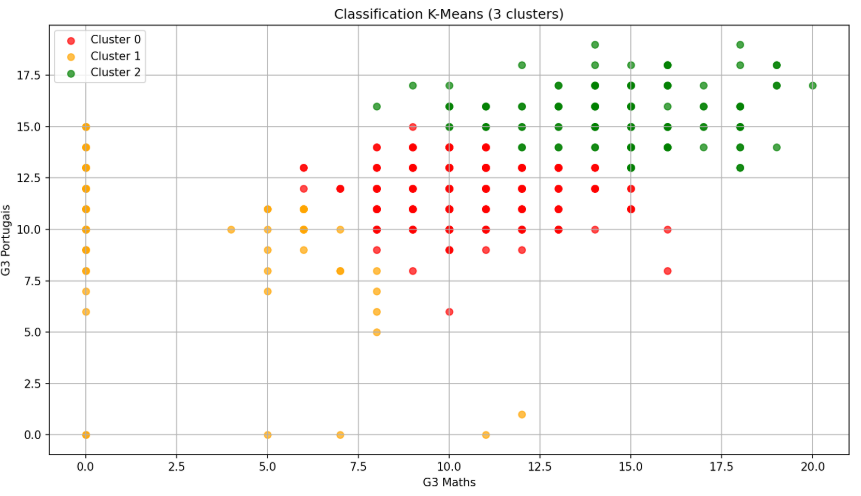
\includegraphics[width=0.57\columnwidth]{figures_rapport/kmeans_notes.png}
\caption{Profils construits à partir de \texttt{G3.x} et \texttt{G3.y}.}
\label{fig:kmeans}
\end{figure}

L'ACP donne ensuite une lecture globale des relations entre variables. Sur le cercle des corrélations, \texttt{Medu} et \texttt{Fedu} sont proches, tout comme \texttt{Dalc.x} et \texttt{Walc.x}. L'axe principal oppose globalement \texttt{G3.x}, \texttt{Medu}, \texttt{Fedu} à \texttt{failures.x}, \texttt{age}, \texttt{absences.x}, \texttt{Dalc.x} et \texttt{Walc.x}. On retrouve donc une opposition entre réussite scolaire, contexte familial favorable et facteurs de risque.

\begin{figure}[H]
\centering
\includegraphics[width=0.70\columnwidth]{figures_rapport/acp_cercle.pdf}
\caption{ACP descriptive: relations entre les variables du jeu de données.}
\label{fig:acp}
\end{figure}

Cette ACP ne prouve pas de causalité, mais elle montre que les variables de contexte ne sont pas indépendantes du niveau scolaire. Elle justifie ensuite l'idée de travailler avec des axes factoriels: au lieu de garder toutes les variables explicatives séparément, on peut projeter l'information sur des composantes principales afin de réduire la dimension et de limiter la colinéarité.

\section{Modèles supervisés sur variables brutes}

La première série de modèles utilise directement les variables de contexte. Deux familles d'arbres sont comparées. La forêt aléatoire construit plusieurs arbres indépendants et agrège leurs décisions, ce qui réduit le surapprentissage. XGBoost construit au contraire les arbres de manière séquentielle: chaque nouvel arbre corrige une partie des erreurs précédentes. Cette méthode peut être très efficace, mais elle demande souvent plus de données pour exploiter pleinement son potentiel.

En régression, l'objectif est de prédire \texttt{G3}. La forêt aléatoire obtient $R^2=0{,}223$ et $\mathrm{MAE}=3{,}04$, tandis que XGBoost obtient $R^2=0{,}105$ et $\mathrm{MAE}=3{,}31$. Le RMSE est proche de 4 points. Ces valeurs indiquent que les modèles se trompent en moyenne d'environ trois points sur 20 et expliquent peu la variance des notes.

\begin{figure}[H]
\centering
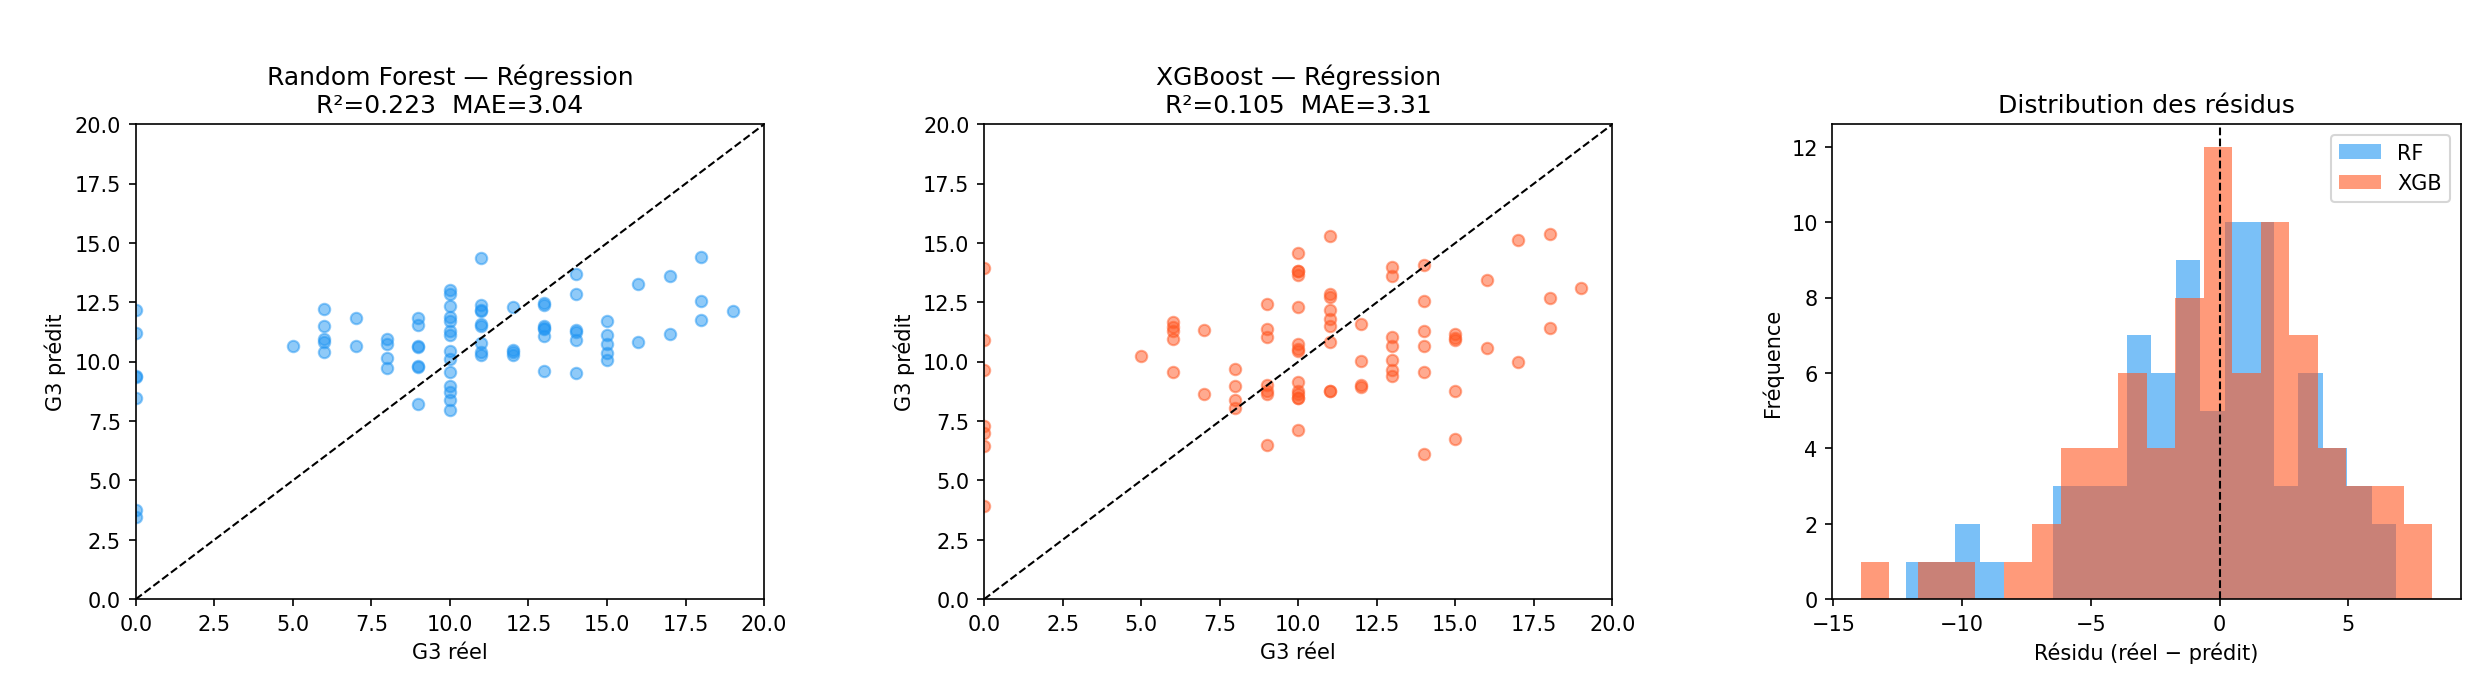
\includegraphics[width=\columnwidth]{figures_rapport/regression_arbres.png}
\caption{Prédiction de \texttt{G3} avec variables brutes: les prédictions restent tassées autour de la moyenne.}
\label{fig:regbrut}
\end{figure}

En classification réussite/échec, les performances sont meilleures mais restent modérées. La forêt aléatoire atteint 67{,}09 \% d'exactitude et une AUC de 0{,}643. XGBoost atteint 62{,}03 \% d'exactitude et une AUC de 0{,}558. L'AUC est importante ici: elle mesure la capacité du modèle à attribuer un score plus élevé à un élève qui réussit qu'à un élève qui échoue. Une AUC de 0{,}643 signifie que ce classement est correct dans environ 64{,}3 \% des comparaisons.

\begin{figure}[H]
\centering
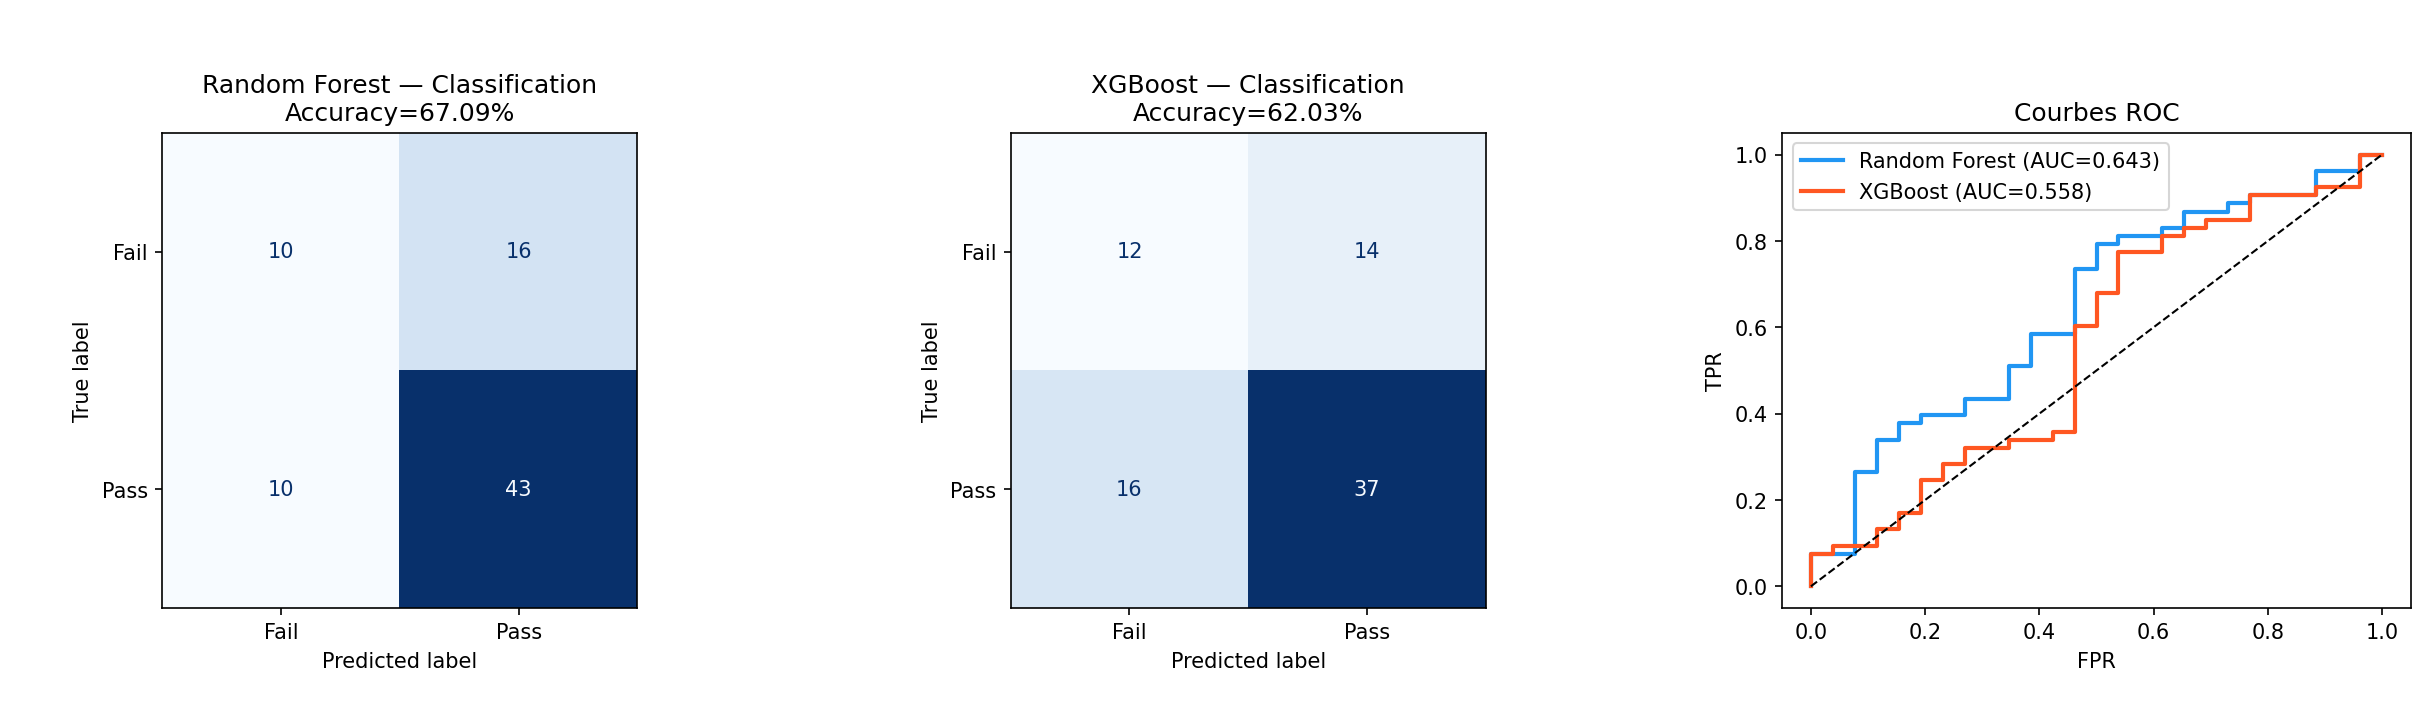
\includegraphics[width=\columnwidth]{figures_rapport/classification_arbres.png}
\caption{Classification réussite/échec avec variables brutes: matrices de confusion et ROC.}
\label{fig:classbrut}
\end{figure}

Les matrices de confusion montrent que les modèles détectent mieux les réussites que les échecs. La forêt aléatoire prédit correctement 43 réussites, mais classe aussi 16 échecs comme réussites. Le modèle est donc davantage un outil de détection imparfaite du risque qu'un outil fiable de décision individuelle.

\section{Facteurs ressortant des arbres}

L'intérêt des arbres est aussi de repérer les variables les plus utilisées. Les deux variables dominantes sont \texttt{failures} et \texttt{absences}. Pour la forêt aléatoire, elles ressortent très nettement devant les autres variables. XGBoost fait aussi apparaître \texttt{failures}, puis \texttt{guardian\_other}, \texttt{higher} et \texttt{absences}.

\begin{figure}[H]
\centering
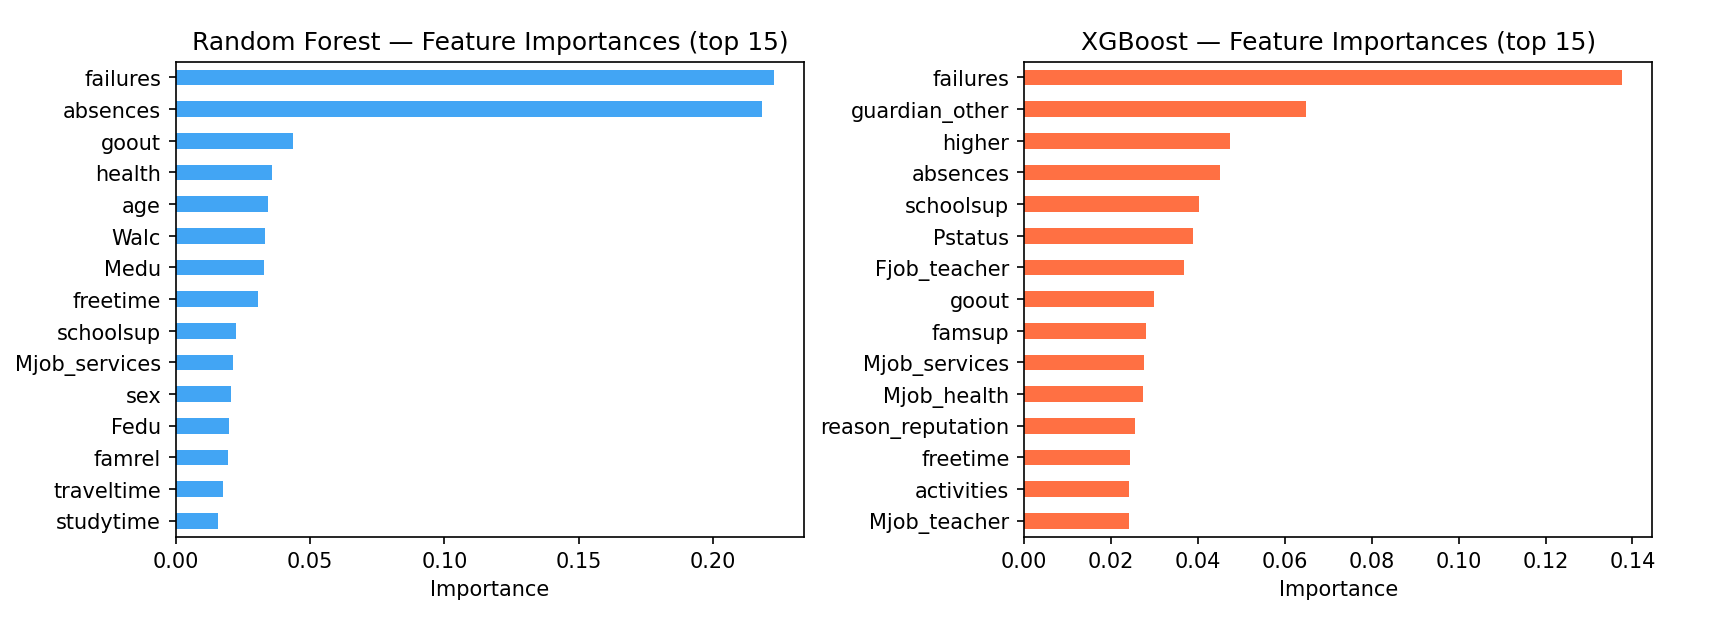
\includegraphics[width=\columnwidth]{figures_rapport/importance_arbres.png}
\caption{Importance des variables dans les modèles d'arbres.}
\label{fig:importance}
\end{figure}

Ces résultats sont cohérents: \texttt{failures} mesure les échecs antérieurs, donc un historique de difficulté; \texttt{absences} mesure l'assiduité. En revanche, une importance élevée ne donne pas le sens de l'effet et ne prouve pas une causalité. Elle indique seulement qu'une variable aide le modèle à réduire ses erreurs de séparation.

\section{Modèles supervisés après projection ACP}

Dans la seconde série d'essais, cette projection est appliquée aux variables explicatives utilisées par les modèles. Les variables sont standardisées puis remplacées par des composantes principales. Il faut 7 axes pour conserver 90 \% de la variance, ce qui montre que l'information n'est pas concentrée dans quelques dimensions seulement. Cela s'explique par la nature des données: beaucoup de variables sont binaires ou issues d'un encodage one-hot, ce que l'ACP comprime moins bien que des variables continues corrélées.

Avec ces axes ACP, la régression devient moins bonne pour les arbres: la forêt aléatoire passe de $R^2=0{,}223$ à $R^2=0{,}070$, avec une MAE de 3{,}30. XGBoost obtient même un $R^2$ négatif ($-0{,}036$), ce qui confirme que la prédiction précise de \texttt{G3} est très fragile sans \texttt{G1} et \texttt{G2}.

\begin{figure}[H]
\centering
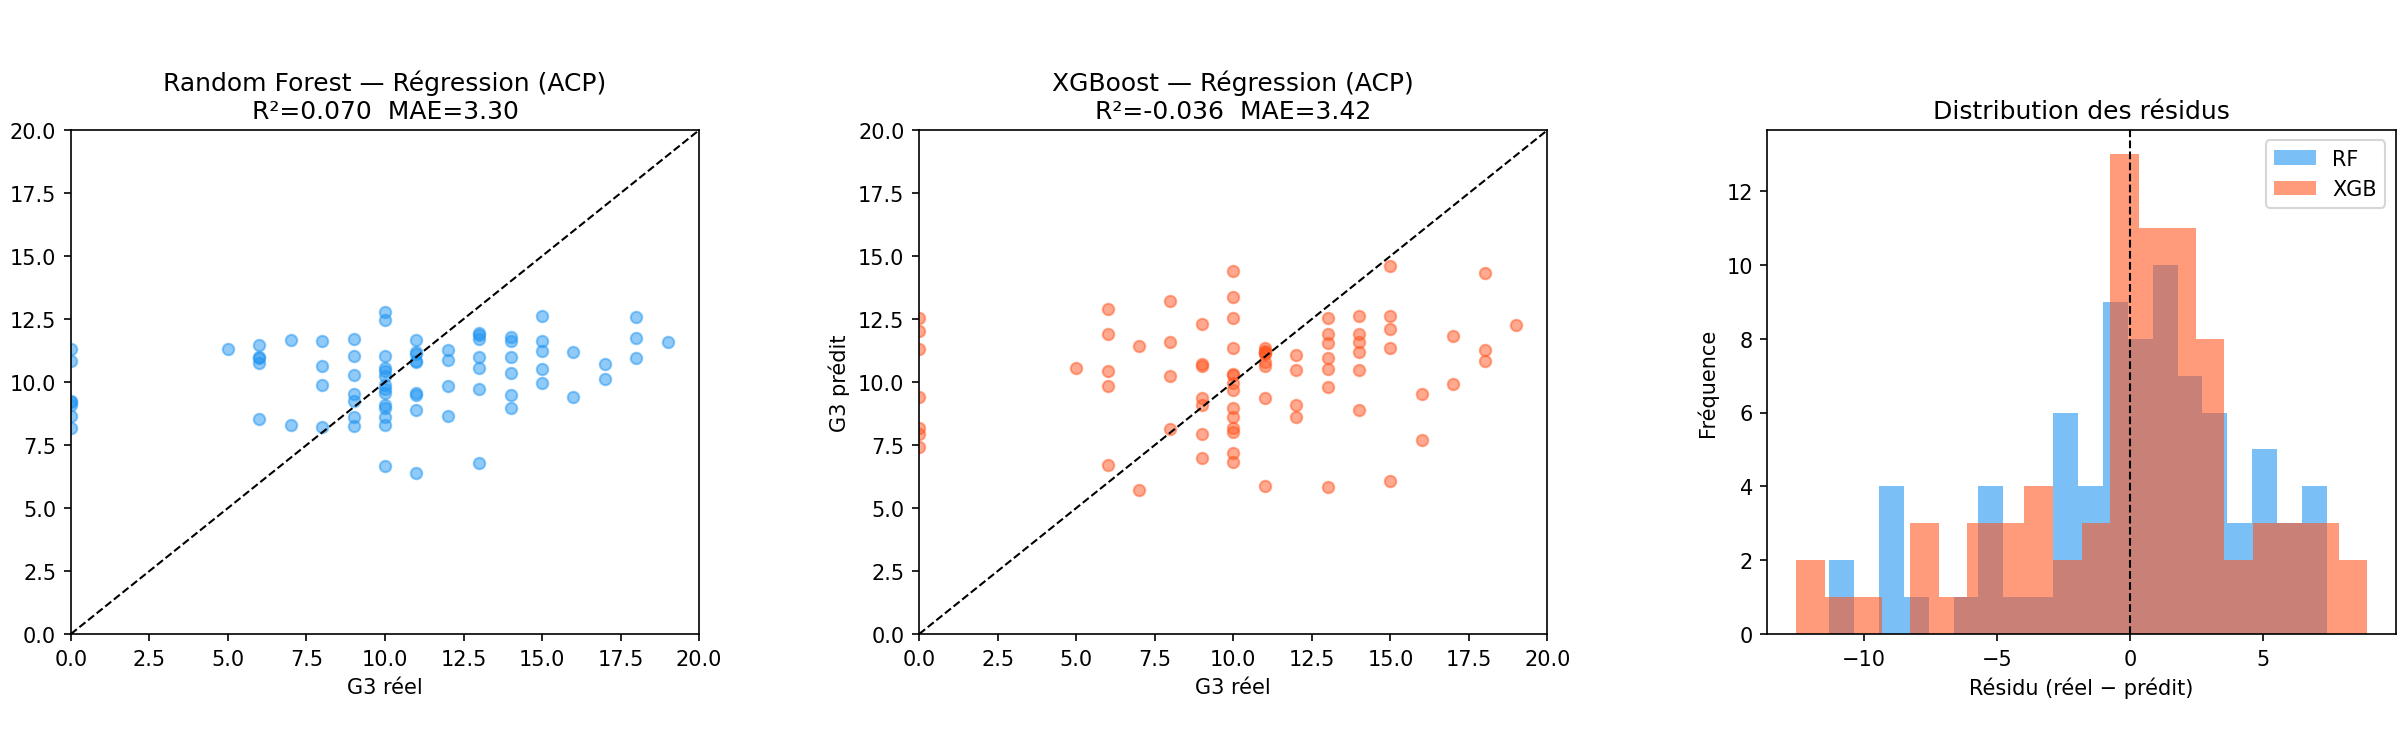
\includegraphics[width=\columnwidth]{figures_rapport/regression_acp.png}
\caption{Régression avec axes ACP: la perte d'information pénalise surtout la prédiction exacte de \texttt{G3}.}
\label{fig:regacp}
\end{figure}

Pour la classification, le passage aux axes ACP donne une conclusion plus nuancée. La régression logistique progresse: son exactitude passe de 55{,}7 \% à 60{,}76 \%, et son AUC de 0{,}598 à 0{,}611. Les arbres, eux, restent stables ou augmente légèrement: la forêt aléatoire passe de 67{,}0 \% à 68{,}35 \% d'exactitude, et son AUC de 0{,}643 à 0{,}546.

\begin{figure}[H]
\centering
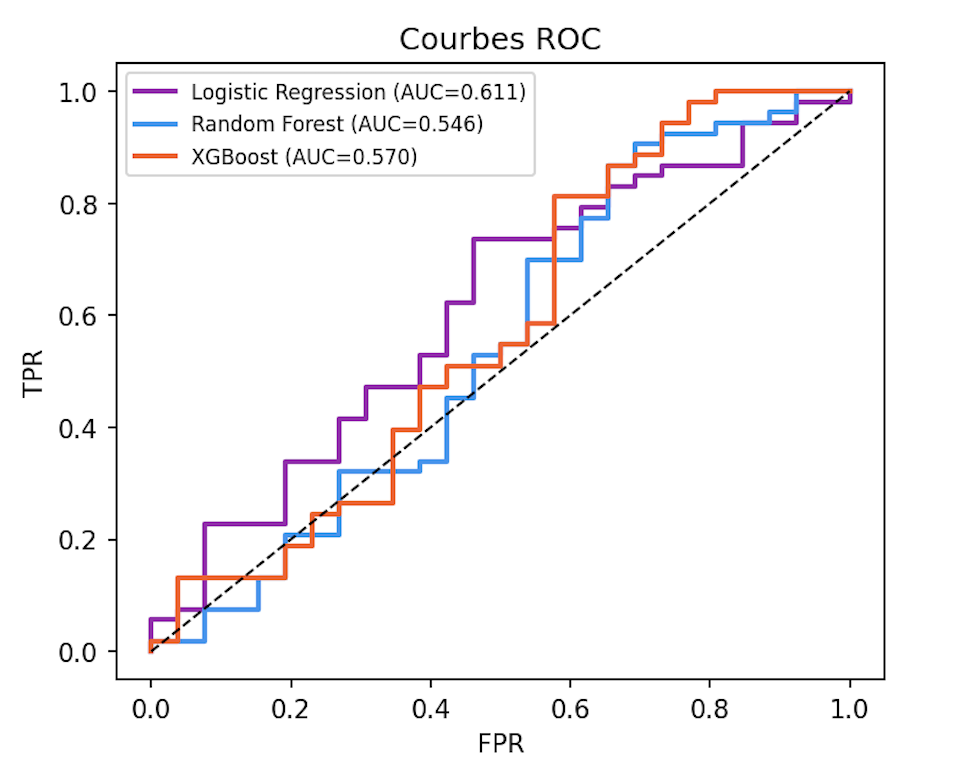
\includegraphics[width=0.72\columnwidth]{figures_rapport/classification_acp_roc.png}
\caption{ROC des modèles de classification entraînés sur les axes ACP.}
\label{fig:rocacp}
\end{figure}

\begin{table}[H]
\centering
\small
\begin{tabular}{lcc}
\toprule
Indicateur & Variables brutes & Axes ACP \\
\midrule
$R^2$ RF régression & 0{,}223 & 0{,}070\\
Accuracy RF & 67{,}0 \% & 68{,}35\%\\
AUC RF & 0{,}643 & 0{,}546\\
Accuracy LogReg & 55{,}7 \% & 60{,}76 \%\\
AUC LogReg & 0{,}598 & 0{,}611\\
Accuracy XGBoost & 62{,}0 \% & 68{,}35 \%\\
\bottomrule
\end{tabular}
\caption{Comparaison variables brutes / axes ACP.}
\label{tab:acp}
\end{table}

Ce résultat est important pour l'interprétation. L'ACP aide un modèle linéaire comme la régression logistique, car elle décorrèle les entrées. Elle apporte aussi un gain aux arbres, qui gèrent déjà assez bien les corrélations et les interactions. L'ACP est donc utile pour stabiliser et résumer, et  améliore dans notre cas la prédiction, bien que ce ne soit pas automatique.

La régression logistique sur variables brutes reste toutefois utile pour lire le sens des associations. Les coefficients négatifs les plus marqués concernent \texttt{failures}, \texttt{goout} et \texttt{schoolsup}: ils sont associés à une probabilité plus faible de réussite. L'interprétation de \texttt{schoolsup} doit rester prudente, car il s'agit probablement d'un effet de sélection: les élèves qui reçoivent du soutien sont souvent déjà en difficulté. À l'inverse, \texttt{higher}, \texttt{studytime} et \texttt{Medu} sont associés positivement à la réussite. Ces coefficients ne prouvent pas une causalité, mais ils donnent des tendances plus lisibles que les importances d'arbres.

\section{Interprétation des axes ACP}

Le passage aux composantes principales modifie aussi l'interprétation des modèles. Avec les variables brutes, on peut dire directement que \texttt{failures} ou \texttt{absences} sont importantes. Avec l'ACP, les modèles utilisent des axes \texttt{PC1}, \texttt{PC2}, etc. Ces axes sont des combinaisons de variables: ils réduisent la dimension, mais ils rendent la lecture moins immédiate.

\begin{figure}[H]
\centering
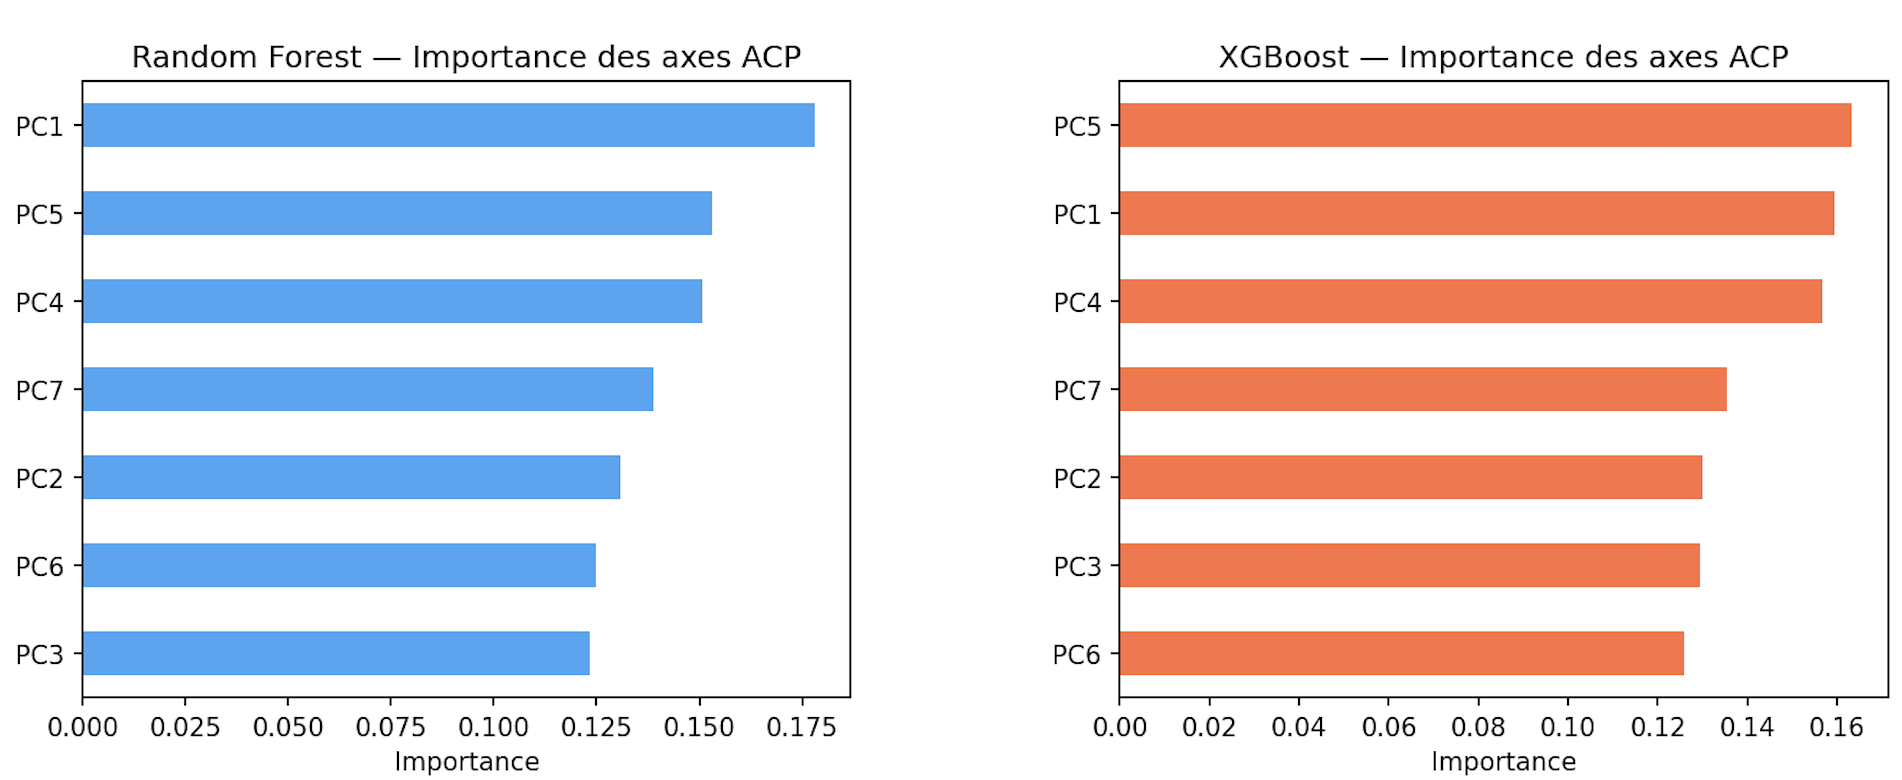
\includegraphics[width=\columnwidth]{figures_rapport/importance_axes_acp.png}
\caption{Importance des composantes principales dans la forêt aléatoire et XGBoost.}
\label{fig:pcimportance}
\end{figure}

Les composantes les plus utilisées ne sont pas seulement les premières. PC1 et PC2 sont mathématiquement garantis d'être les deux axes qui portent le plus d'inertie (de variance), mais le plus de variance ne veut pas dire le plus pertinent pour notre question, si bien que les deux modèles accordent une forte importance à \texttt{PC5} et \texttt{PC4}, et donc l'information utile pour la classification est dispersée dans plusieurs dimensions, pas uniquement dans \texttt{PC1} et \texttt{PC2}. La forêt aléatoire utilise aussi fortement \texttt{PC1}, tandis que XGBoost met aussi en avant des axes comme \texttt{PC5}. D'après l'analyse des poids des axes, \texttt{PC1} correspond surtout à un axe lié au contexte familial et scolaire, avec \texttt{Medu}, \texttt{Fedu}, \texttt{higher}, mais aussi une opposition avec \texttt{age} et \texttt{failures}. \texttt{PC2} est davantage lié aux comportements sociaux, avec \texttt{Dalc}, \texttt{Walc} et \texttt{goout}.

Cette étape explique pourquoi l'ACP donne des résultats ambivalents. Elle peut aider la régression logistique, car ce modèle linéaire profite aux variables décorrélées. 

\section{Analyse discriminante après ACP}

L'analyse discriminante est appliquée sur les composantes principales. QDA est régularisée, avec un meilleur paramètre \texttt{reg\_param = 0.4}. En validation croisée, la meilleure zone est autour de 0{,}7185 d'exactitude, ce qui correspond à un compromis entre stabilité des covariances et flexibilité.

\begin{figure}[H]
\centering
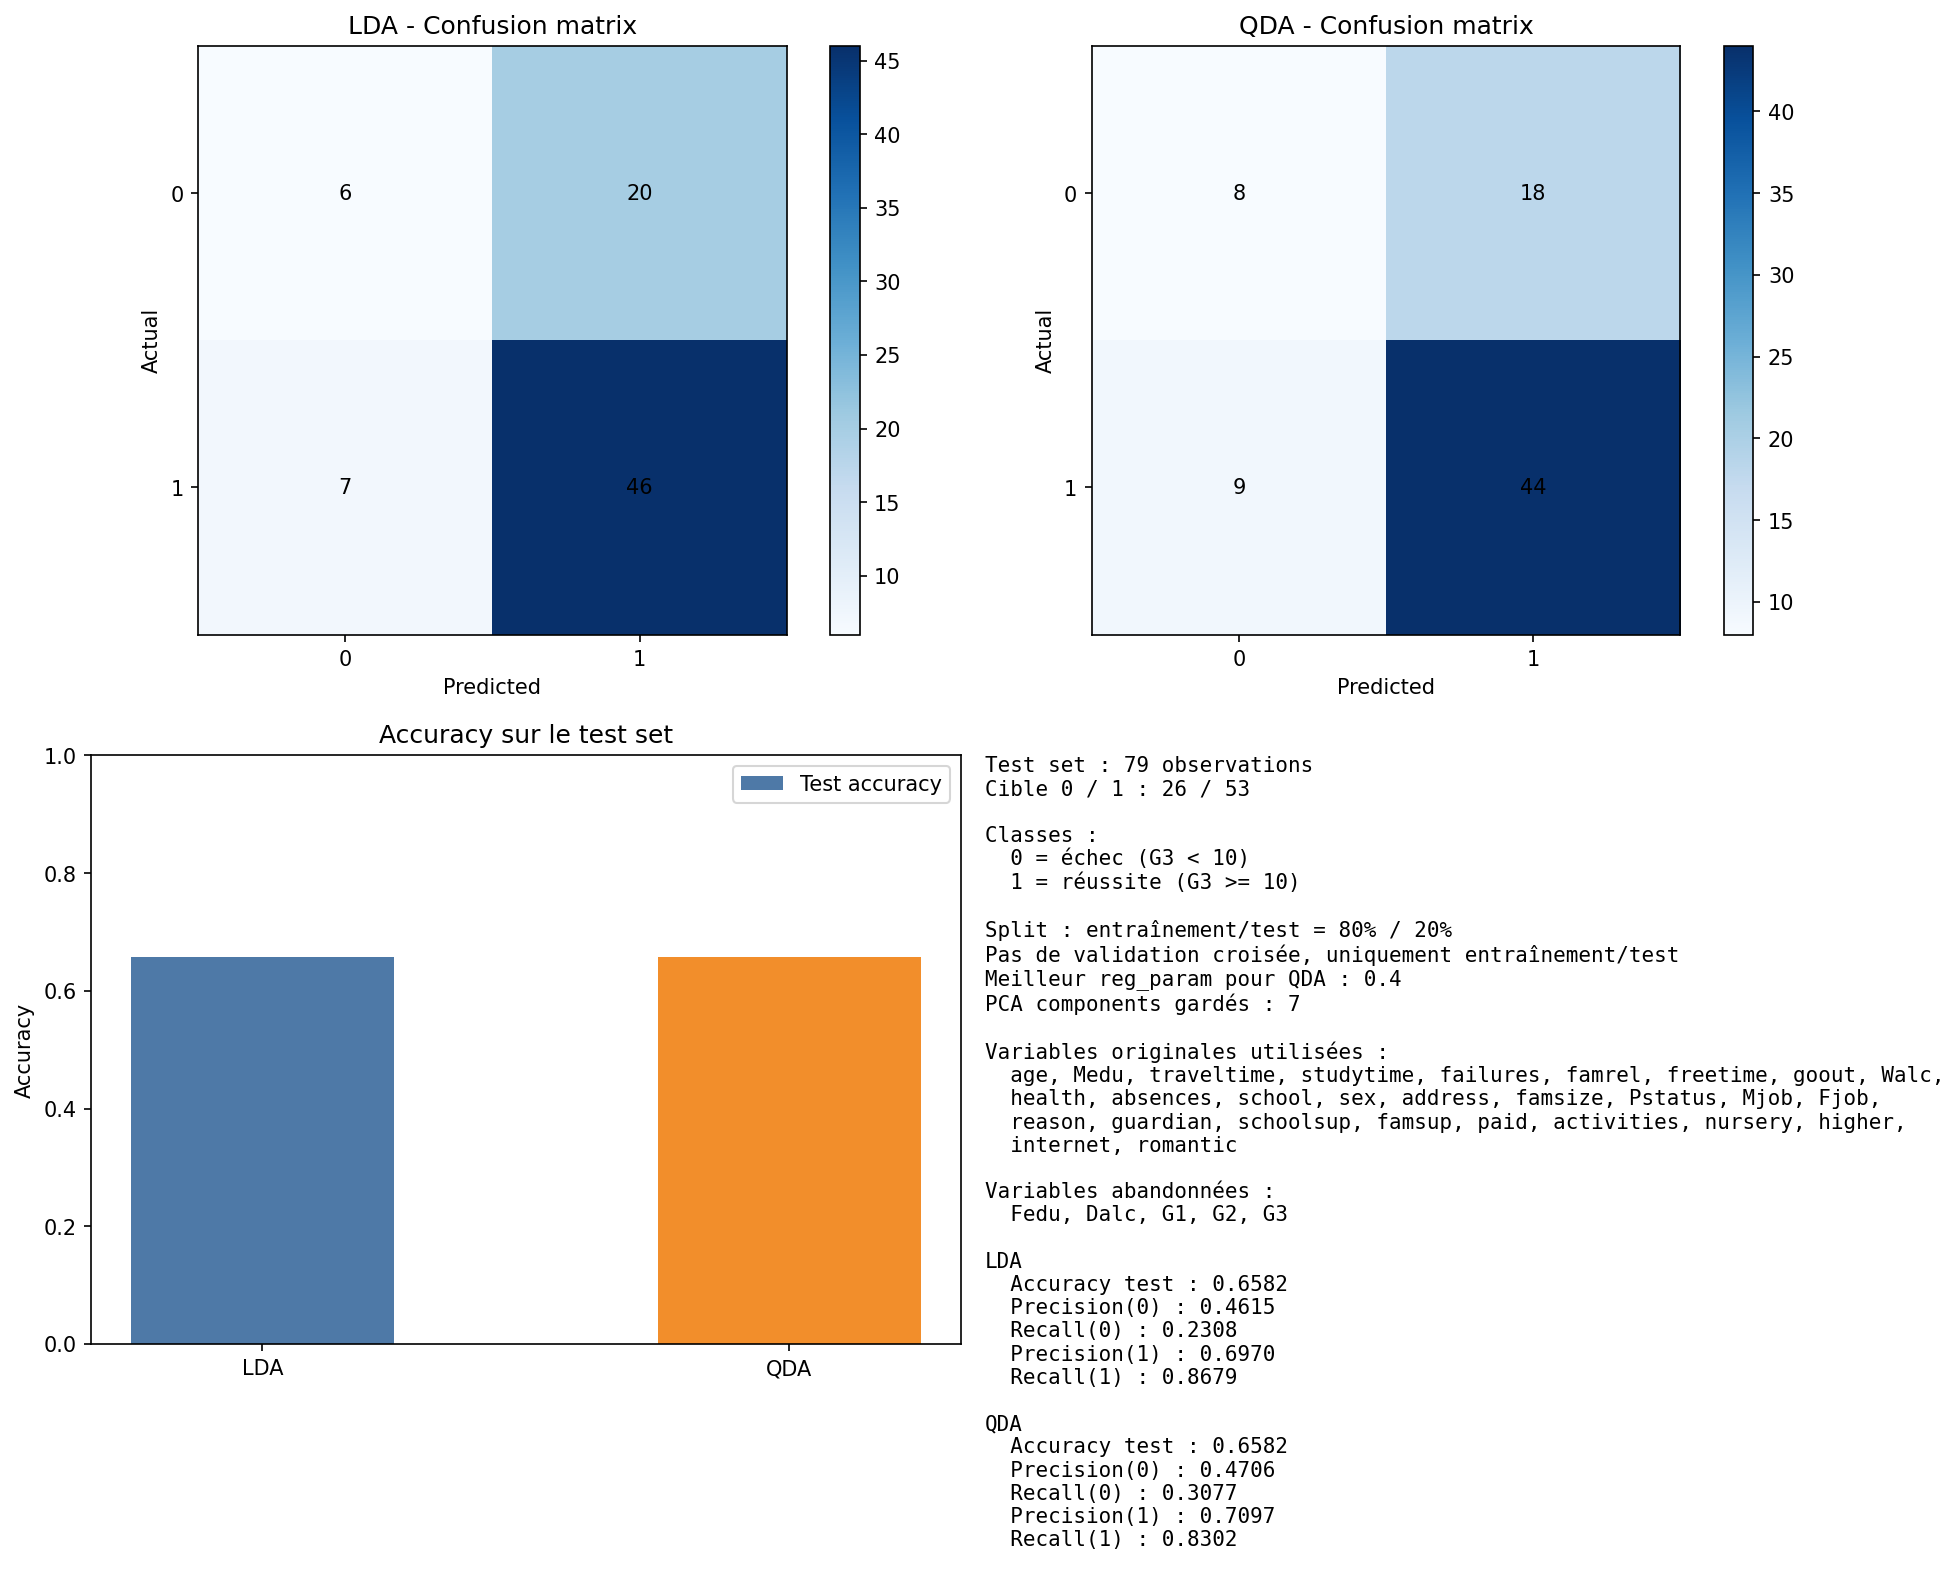
\includegraphics[width=0.92\columnwidth]{figures_rapport/discriminante_acp.png}
\caption{Analyse discriminante après ACP: LDA et QDA donnent une exactitude proche sur le test.}
\label{fig:disc}
\end{figure}

Sur le jeu de test, LDA et QDA obtiennent la même exactitude globale, environ 65{,}82 \%. La différence est dans la répartition des erreurs: QDA détecte légèrement mieux les échecs, mais perd quelques réussites. Cela suggère que la structure est légèrement non linéaire, sans gain suffisant pour obtenir une séparation nette entre les classes.

\section{Conclusion}

Les résultats répondent aux deux questions initiales. D'abord, on ne prédit pas précisément la note finale avec les variables de contexte seules: les $R^2$ restent faibles et les erreurs moyennes dépassent trois points. Les modèles ramènent souvent les prédictions vers des notes moyennes, ce qui confirme que les variables disponibles ne suffisent pas à expliquer la variabilité fine de \texttt{G3}.

Ensuite, la classification réussite/échec fonctionne mieux que la prédiction exacte de la note, mais reste modérée. La forêt aléatoire est le modèle le plus convaincant sur les variables brutes, avec environ 67 \% d'exactitude et une AUC proche de 0{,}64. Elle permet donc de repérer un risque scolaire mieux que le hasard, mais elle ne constitue pas un outil fiable de décision individuelle. Les modèles détectent surtout mieux les élèves en réussite que les élèves en échec, ce qui montre que les profils d'élèves en difficulté sont moins bien caractérisés par les variables disponibles.

Le projet met aussi en évidence des facteurs récurrents: \texttt{failures} et \texttt{absences} ressortent fortement dans les arbres, tandis que la régression logistique rend plus lisibles certaines tendances associées à \texttt{goout}, \texttt{schoolsup}, \texttt{higher}, \texttt{studytime} ou \texttt{Medu}. Ces résultats doivent rester interprétés comme des associations, et non comme des causalités.

Enfin, le passage par ACP apporte surtout un intérêt méthodologique. Il réduit la dimension, décorrèle les variables et améliore légèrement la régression logistique, mais il n'améliore pas globalement les arbres. L'analyse discriminante confirme la même idée: LDA et QDA obtiennent une performance équivalente, autour de 66 \%, ce qui suggère une séparation imparfaite et globalement proche d'une structure linéaire. La conclusion générale est donc nuancée: les variables de contexte contiennent bien un signal prédictif, mais ce signal reste insuffisant pour reconstruire précisément le niveau scolaire sans les notes intermédiaires \texttt{G1} et \texttt{G2}.

\end{document}
